%
%  This is an example LaTeX file. The percent sign is used to mark the
% start of a comment.
%
%  - Michael Weeks,  January, 2003
%
\documentclass[conference]{IEEEconf}
\usepackage{rotating,graphicx}
\usepackage[hidelinks]{hyperref}
\hypersetup{
  colorlinks   = true,    % Colours links instead of ugly boxes
  urlcolor     = blue,    % Colour for external hyperlinks
  linkcolor    = blue,    % Colour of internal links
  citecolor    = red      % Colour of citations
}

%\journal{CSc 4110 Final Report}

%\title[journalExample]{Format for Project Reports}
\title{Engineering Update on the project: \textit{\textbf{"EEG Measures for Schizophrenia"}}}
% \author{%
% Dr. K.P. Ayodele, Emmanuel OLATEJU \\
%     \begin{affiliation}
%       Excelsiors \\ 09/02/2023, \\
%       email: \mbox{kayodele@gmail.com, eoolateju@student.oauife.edu.ng}
%       \end{affiliation}
% }


\begin{document}



\maketitle


\begin{abstract}
  Significant improvements have been made in the Generis software used for acquisition. Some of the changes include stimuli and instruction presentation to patient, and
  changes are being made to allow for module expansion for annotation flexibility.

  Also, data processing has evolved overtime and has involved montage, time-series plots and more recently analysis is rich enough to monitor frequency evolution over time using the
  short time fourier transform.

  Also, a brief computational analysis has been carried out on the data of 32 subjects as suggested by the clinicians to check data-integrity before furthering data acquisition. 
  Previous data analysis was blind to some patient charactersitics such as age, gender, language. This has currently been resolved. Also new data analysis pipeline 
  have been developed to allow for future expansion of features through the use of pipeline and transformers technology.

  Computational analysis was carried out to investigate the presence of mismatch negativity and other EEG features that are discriminative of the SZ populace and the control subjects.
  The results of the controls are presented first before that of the SZ populace.
\end{abstract}

\section{Introduction}\label{sec:intro}
An already implemented workflow architecture for the project was presented and its results on dummy(not-simulated) data was shown 
including the binary classifiers results. Currently withing the workflow architecture, the pre-proessing pipeline
has been update to cater for needs in comparing different preprocessing steps. Figure \ref{fig:preprocessPipeline} shows the 
new preprocessing pipeline.

The Generis-V6 version of the custom made Generis software was used in the data acquisition and all processed data was from the contec-KT2400.
Annotation was rigid and was not adaptable. Annotations have evolved overtime and is currently being updated to cater for patient 
and clinician input during the course of recording.

Previously, results of a basic data-preprocessing and processing pipeline were presented. This included montage plots, and EEG time-series plot of various
cortical regions intended to show mismatch negativity response to the auditory stimuli. The data was from the first three subjects of which, one was male and two female.
An already improved analysis has been achieved showing the time-response plots of the temporal lobes,
the spectrogram differences across the four phases of EEG aquisition and the entropy differences across
various brain regions \textit{(Frontal/Frontal-parietal, Parietal/Central, Parietal/Occipital and Temporal/Occipital) lobes}.

This report will give a summary on the 32 subjects acquired data and then present the progress made so far and changes being made as follows:
  \begin{itemize}
    \item Generis stimuli presentation
    \item Generis annotation
    \item Analysis
  \end{itemize}
Then this report will present a plate summary of new analytial results on acquired data, and the next set of action points.

\section{Data Summary}
Certain brickwalls were encountered during data-processing due to unavoided faults in data acquisition. These faults include:
\begin{itemize}
  \item Non-uniform time for phases across patients
  \item Non-uniform number of trials
  \item Incomplete phases in certain trials
  \item Certain device inconsistency
  \item Wrong sampling frequency selection, due to wrong device selection.
\end{itemize}
Overall, data acquisition needs to be improved. Some data sessions and trials have ertain faults that
leads to their being shunned.
Faulty data is mostly due to human error expressed as inconsistency in decisions of recording
parameters and mostly manifest in one or two trials of very little number of subjects.

These subjects id's will have their recording parameters investigated as one or more of their
recordings were null, thus having no analysis results. Their info is given below:

\textit{
  {'16': {'rest1': [0, 1], 'arith': [0, 1], 'rest2': [0, 1], 'auditory': [0, 1]}, '20': {'rest1': [], 'arith': [], 'rest2': [], 
'auditory': [0]}, '23': {'rest1': [], 'arith': [0], 'rest2': [0], 'auditory': [0]}, '32': {'rest1': [0, 1, 2], 'arith': [0, 1, 2],
 'rest2': [0, 1, 2], 'auditory': [0, 1, 2]}, '4': {'rest1': [], 'arith': [], 'rest2': [2], 'auditory': [2]}, '5': {'rest1': [0, 1], 
 'arith': [0, 1], 'rest2': [0, 1], 'auditory': [0, 1]}, '6': {'rest1': [], 'arith': [], 'rest2': [], 'auditory': [0]}, '8': {'rest1': 
 [0, 1], 'arith': [0, 1], 'rest2': [0, 1], 'auditory': [0, 1]}, '9': {'rest1': [0, 1], 'arith': [0, 1], 'rest2': [0, 1], 'auditory': [0, 1]}}
}

Ignoring \textit{subject '1'} which is a dummy profile used in testing the software, 
there were a total of 18 patients and 13 control, after ignoring the subjects with null data 
as shown above, there were 10 patients and 12 control subjects on which data analysis results
were obtained.
            
\section{Progress}
\subsection{Generis Stimuli Presentation}
Previous Generis versions presented stimuli in a static and non-flexible manner. Stimuli was presented in non-auditory phases via the Generis patient interface in 
a textual manner which was language restricted(English). The acquisition paradigm entails a first rest, arithmetic task, second rest and auditory stimuli.

Auditory stimuli presentation remains the same in the presentation of standard and deviant tones, with focus deflecting visuals presentation.This requires no language
considerations.

Rather than presenting instructions in just the english language, since data acquisition requires knowing the spoken language of the subject, efforts have been made
to have instructions written in the yoruba language, other languages yet to be addressed.

More importantly, in the latest version of Generis software, V10, audio recordings of the instructions for the arithmetic task phase has been incorporated
into the software for english, youruba, hausa and pidgin languages.

\subsection{Generis annotation}
Current methods of annotating EEG data with time are rigid and do not permit for user input, user being the patient and clinician.

The auditory stimuli phase is annotated based on the frequency and amplitude charactersitics of presented tone. The rest phases are given an empty
character annotation across all time instances and the same goes for the arithmetic.During the arithmetic, patients need to indicate when they understand the task,
are ready to give their answer and are ready to proceed to the next arithmetic task, this acts as a form of feedback by the patient to the brain computer interface system. 
The clinician in charge of data acquisition also needs to be able to annotate times of 
patient deviation from instructions and artifact introduction by body movements.

The software is currently being expanded to allow for patient and clinician annotation input to the system.

\subsection{Analysis}
The initial analytical pipeline adopted was not robust enough to allow for quick implementation of new processing algorithms as a generic data formating was not designed 
for the purpose of data processing, thus data processing was ignorant of non EEG associated information such as age, gender, language, etc. Also previous processing
methods followed the use of a fixed architecture. With the use of the pipeline and transformers technologies, a new preprocessing pipeline which allows for optional paths and the replacements of optional processors has 
been adopted.

The new processing and analytical methods employs data processing pipeline technology in arranging acquired data into a generic format which memorizes non EEG affiliated
data including the patients name. Using the pipeline technology and transformers technology, new processing alogorithms and modules can be added by implementing a fit
and a transform method for each one. Their class instance and arguments are simply added to the pipeline list for them to be used as processors in the pipeline.

Previous method of analysis presented results in forms of a montage plot and multi-channel time-series. These are shown by figures \ref{fig:ordinary eeg montage} through \ref{fig:MMN time-series plot} 
in section \ref{sec:results} of this document. More recently, analyis has moved to computing the short time fourier transform spectrogram 
of the four phases of data acquisition from the frontal and parietal electrodes and 
computation of the entropy values of the \textit{Frontal/Frontal-parietal, Parietal/Central, Parietal/Occipital and Temporal/Occipital lobes}.
Their results are plotted first for the control subjects and then for the SZ patients.

On the newly acquired data from 32 subjects, the newly developed pipeline and transformers were utilized in pre-processing as follows:
\begin{itemize}
  \item channel dropping
  \item baseline correction
\end{itemize}
Certain channels which do not apply to the scope of this project such as EOG channels were dropped. This was not done in previous data processing. Afterwards baseline
correction was employed by subtracting the average of each channel from each of its time samples. After baseline correction, epoching was carried out.

Per subject analysis was carried out as follows:
To derive the MMN time-series plot, the following was done:
\begin{itemize}
  \item A 100ms epoching from stimuli onset of auditory stimuli class signals.
  \item Averaging of epochs of auditory stimuli class signals.
  \item Time-series plot of resulting auditory stimuli signals in the temporal lobes.
\end{itemize}
To derive the STFT spectrogram, the following was done:
\begin{itemize}
  \item Appropriate epoching of all phases data.
  \item STFT spectrogram computation of epochs.
  \item Averaging of spectrogram epochs of phase.
  \item Extraction of frontal/frontal-parietal eletrodes data from all phases
  \item Averaging of resulting STFT spetrograms of frontal/frontal-parietal electrode sites.
\end{itemize}
To derive the fuuzzy entropy values the following was done:
\begin{itemize}
  \item Extraction of frontal/frontal-parietal, parietal/central, parietal/occipital and temporal/occipital lobes EEG data
  \item Epoching of EEG data across all phases
  \item Averaging of epochs in phases
  \item Computation of fuzzy entropy of resulting data.
\end{itemize}

The results are all shown in figures \ref{fig:rest1 spectrogram_rest1} through \ref{fig:rest1 spetrogram_rest2} 
in section \ref{sec:results} of this document and they show significant difference between the rest phases and the 
arithmetic task phase.

Montage plots indicating the evolution of frequencies of interest overtime are to be developed. These are to be used 
in Auditory Steady State Response studies and entropy studies. Also montage plots showing evolution of temporal region 
overtime are to be developed to better understand the MMN behaviour in controls and patients.

\section{Results}\label{sec:results}
Figure \ref{fig:preprocessPipeline} shows the new preprocessing pipeline with non-filled arrows indicating alternative paths during preprocessing.
Figure \ref{fig:workflow Architecture} shows the workflow architecture which is still being maintained. Currently MMN and ASSR computation modules 
have been implemented.

Fugres \ref{fig:ordinary eeg montage} through \ref{fig:EEG montage with edge and baseline correction} show the different montage resulting from three different preproessing paths. 
Figure \ref{fig:ordinary eeg montage} is from the raw EEG data, while Figure \ref{fig:EEG montage with edge} employs edge interpolation.
Figure \ref{fig:EEG montage with edge and baseline correction} employs edge interpolation and baseline correction.

Figures \ref{fig:MMN time-series plota} and \ref{fig:MMN time-series plot} show the temporal lobe activity of a patient in response to a series of auditory stimuli of standard and deviant tones.
Figure \ref{fig:MMN time-series plota} indicates evenr related potential in response to auditory stimuli in the left temporal region.

Figures \ref{fig:control_11} through \ref{fig:control_31} shows the results of most recent analysis on controls.
Figures \ref{fig:patient_3} trough \ref{fig:patient_25} shows the result of most recent analysis on SZ patients.

\clearpage
\section{Summary}
Signal processing has been implemented to be flexible. Certain considerations discussed
within the \ref{sec:actionPoints} are to be taken to allow for more flexible
and uniform data-acquisition. Time frame for each phase has to be uniform across all subjects
, so also the number of trials for a subject. Focus should be placed on montage presentation 
of data analysis and processing results for purpose of interpretation and feature format for
 algorithms.

\section{Next Steps}\label{sec:actionPoints}
\begin{itemize}
  \item Decide on uniform time of data acquisition for phases and maximum no of trials.
  \item Implement audio stimuli modality for igbo language and rest phases.
  \item Develop annotations for commencement and end of an arithmetic task.
  \item Develop system for patient and clinician input for annotations.
  \item Expand annotation to allow marking of important artifact points by clinician.
  \item Develop algorithm for time evolving frequency montages.
  \item Improve on ASSR module algorithm.
  \item Implement entropy computation modules
\end{itemize}

% \pagebreak
% \newpage
\clearpage
% \subsection{pipelines}
\begin{figure}
  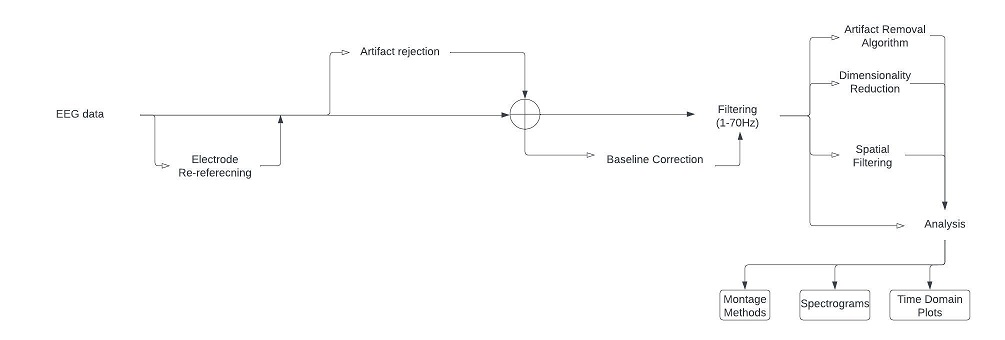
\includegraphics{preProcessing.jpeg}
  \caption{Newly Adopted preprocessing pipeline}
  \label{fig:preprocessPipeline}
\end{figure}
\begin{figure}
  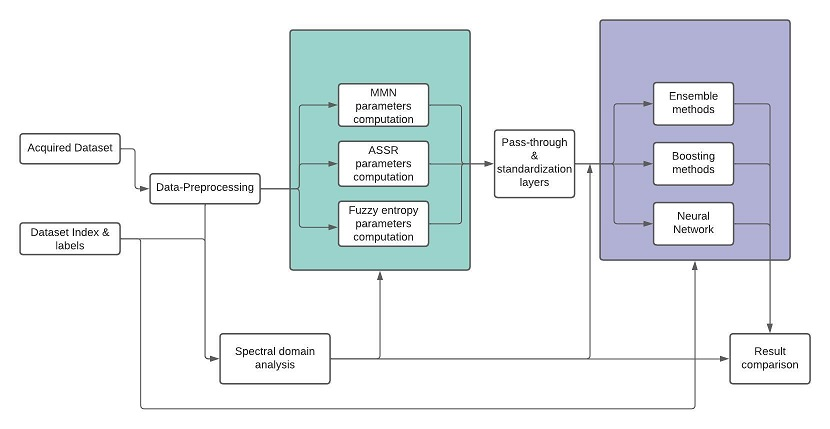
\includegraphics{workflowArchitecture.jpeg}
  \caption{Workflow Architecture}
  \label{fig:workflow Architecture}
\end{figure}

\clearpage
% \subsection{montages}
\begin{figure}
  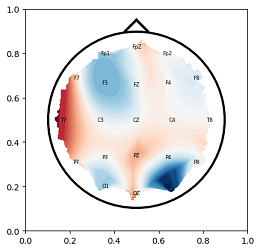
\includegraphics{ordinary_montage.png}
  \caption{Ordinary EEG Montage}
  \label{fig:ordinary eeg montage}
\end{figure}
\begin{figure}
  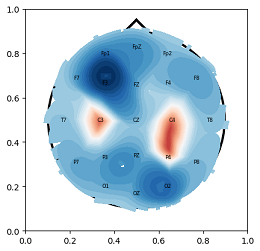
\includegraphics{edge_mean_montage.png}
  \caption{EEG Montage using Edge Interpolation}
  \label{fig:EEG montage with edge}
\end{figure}
\begin{figure}
  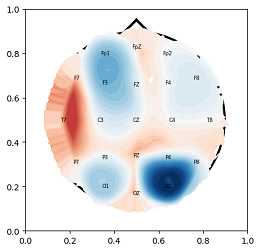
\includegraphics{edge_mean_baseline_montage.png}
  \caption{EEG Montage with baseline correction \& Edge Interpolation}
  \label{fig:EEG montage with edge and baseline correction}
\end{figure}

\begin{figure}
  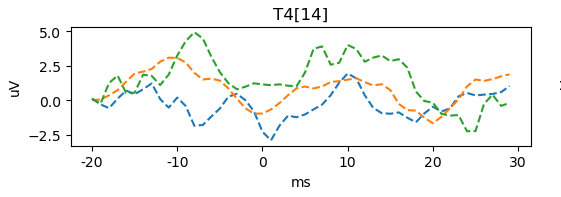
\includegraphics{simiat_temporal.png}
  \caption{Time-Series Plot(MMN) for a patient} 
  \label{fig:MMN time-series plota}
\end{figure}

\begin{figure}
  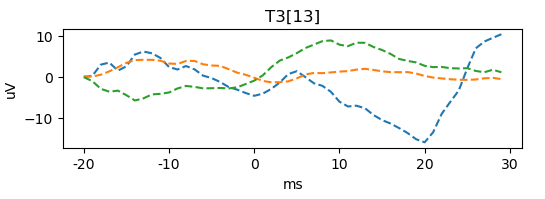
\includegraphics{simiat_temporal1.png}
  \caption{Time-Series Plot(MMN) for a patient} 
  \label{fig:MMN time-series plot}
\end{figure}

\clearpage
% \subsection{pipelines}
\begin{figure}
  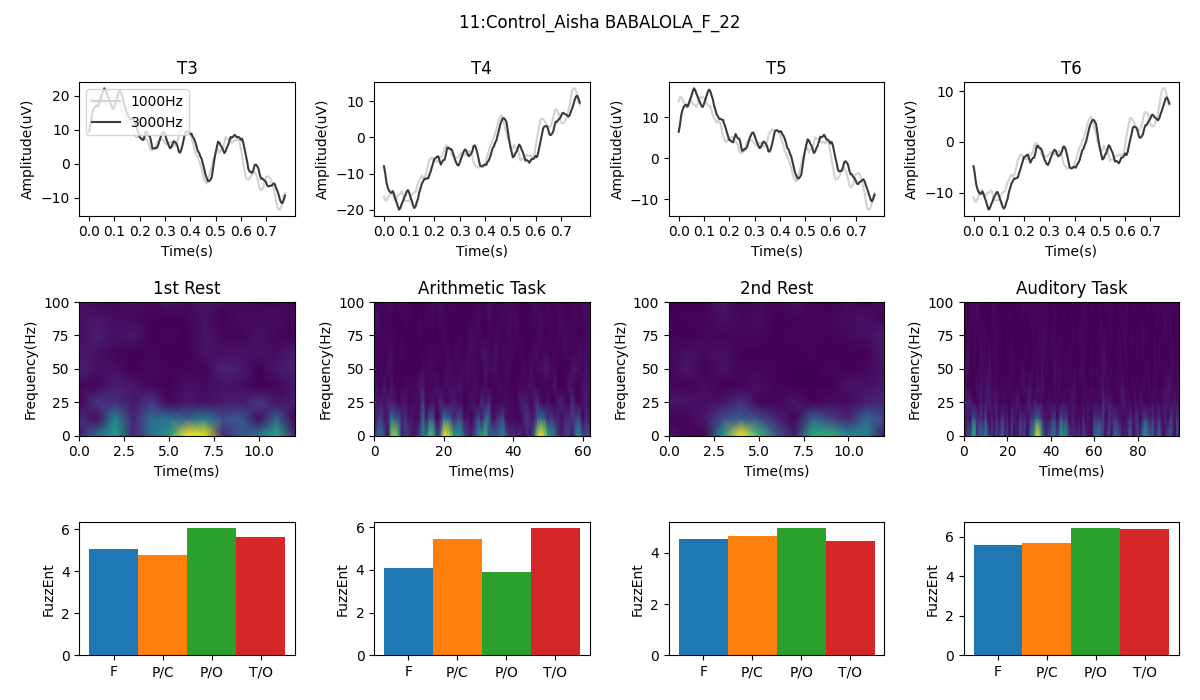
\includegraphics[width=\textwidth]{../../data_analysis_results/results/Control/11.png}
  \caption{Control 11}
  \label{fig:control_11}
\end{figure}
\clearpage
\begin{figure}
  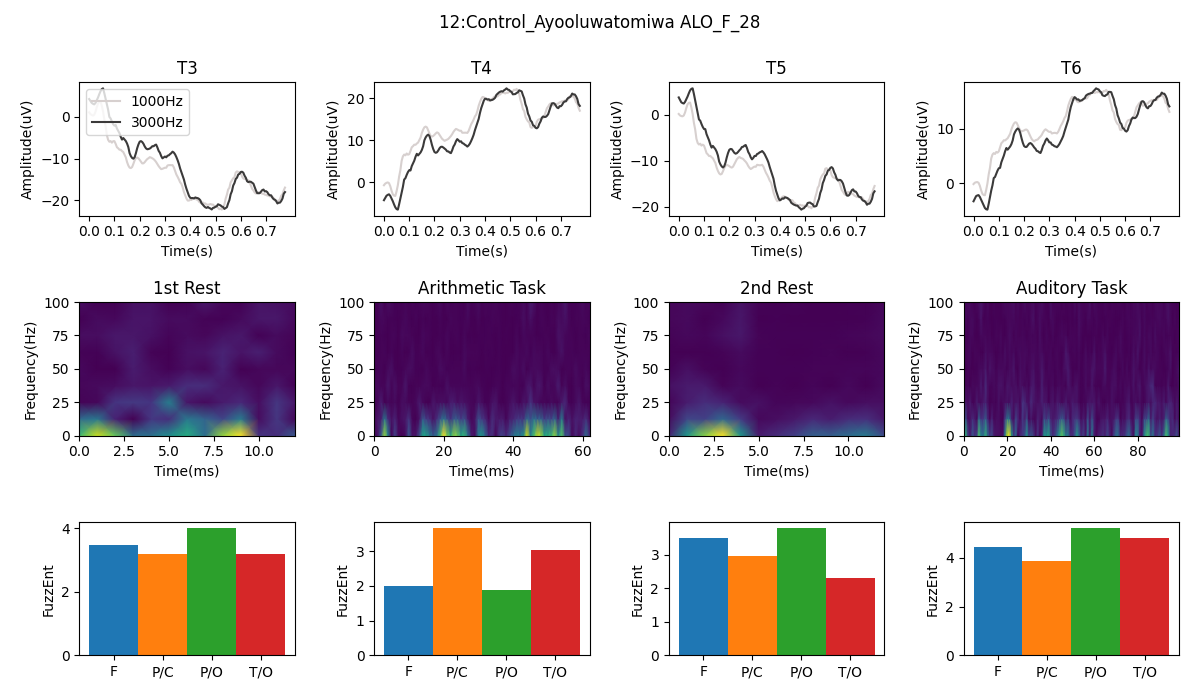
\includegraphics[width=\textwidth]{../../data_analysis_results/results/Control/12.png}
  \caption{Control 12}
  \label{fig:control_12}
\end{figure}
\clearpage
\begin{figure}
  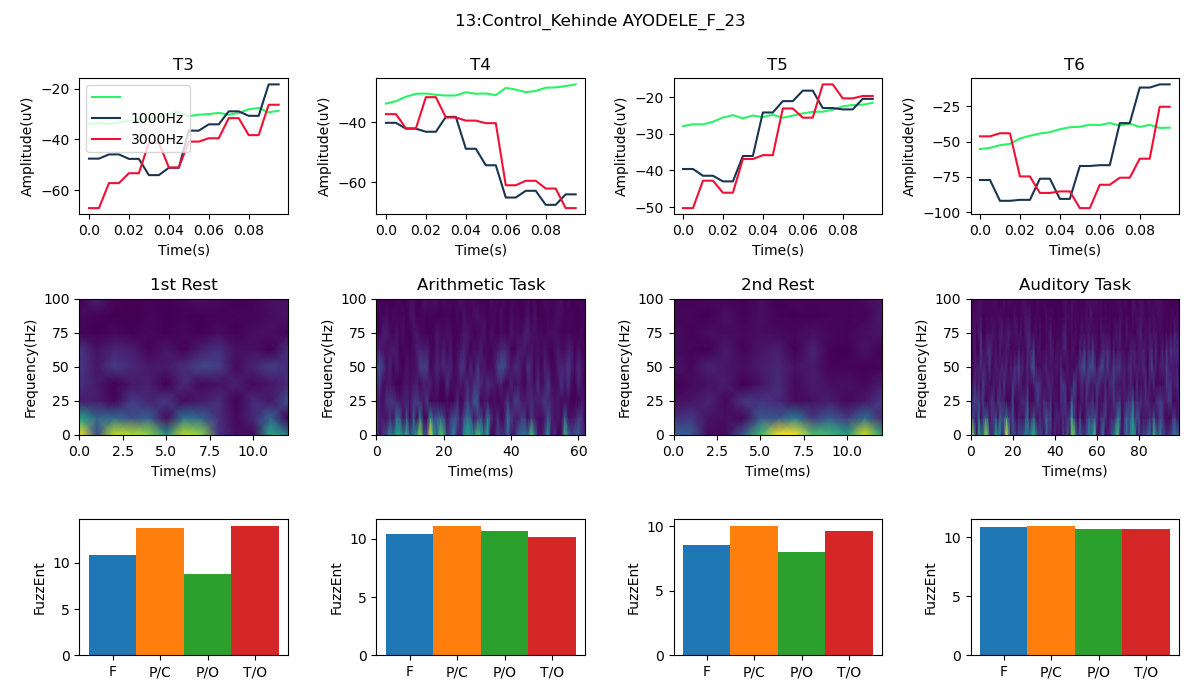
\includegraphics[width=\textwidth]{../../data_analysis_results/results/Control/13.png}
  \caption{Control 13}
  \label{fig:control_13}
\end{figure}
\clearpage
\begin{figure}
  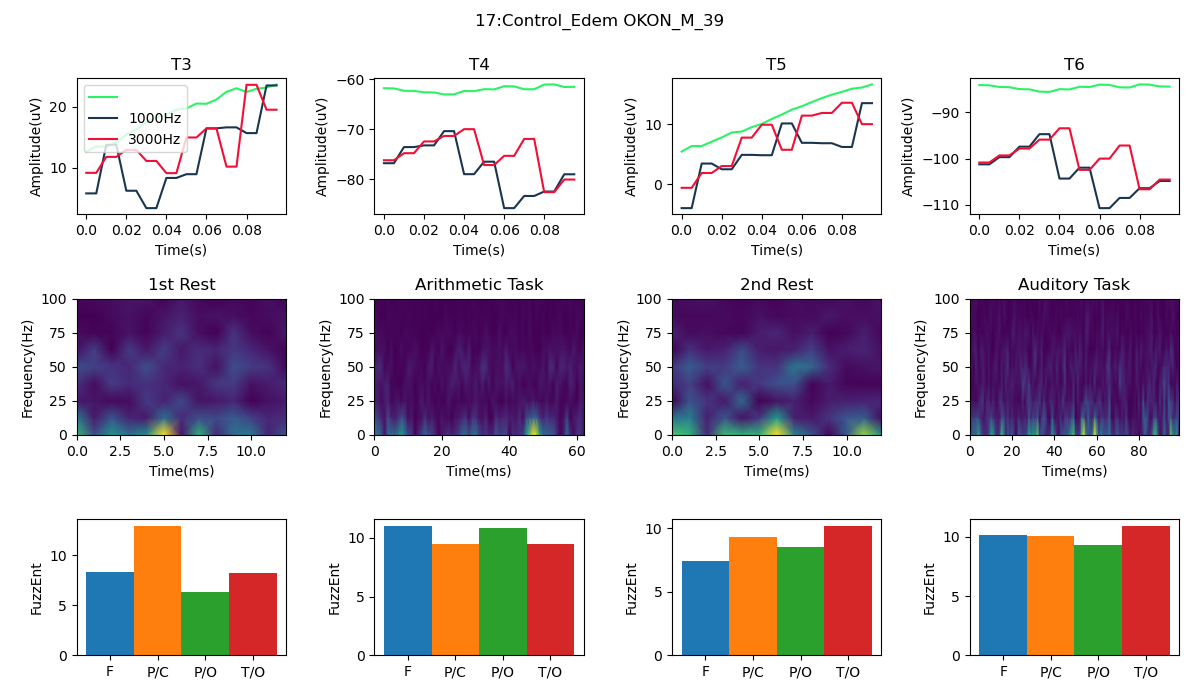
\includegraphics[width=\textwidth]{../../data_analysis_results/results/Control/17.png}
  \caption{Control 17}
  \label{fig:control_17}
\end{figure}
\clearpage
\begin{figure}
  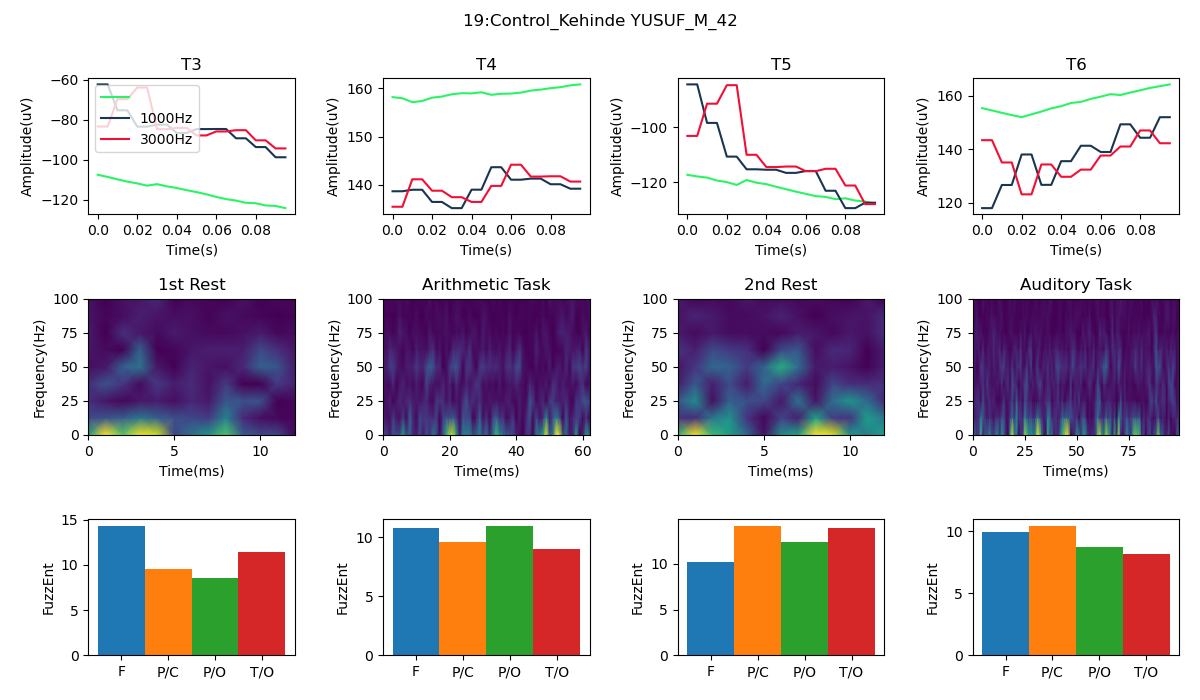
\includegraphics[width=\textwidth]{../../data_analysis_results/results/Control/19.png}
  \caption{Control 19}
  \label{fig:control_19}
\end{figure}
\clearpage
\begin{figure}
  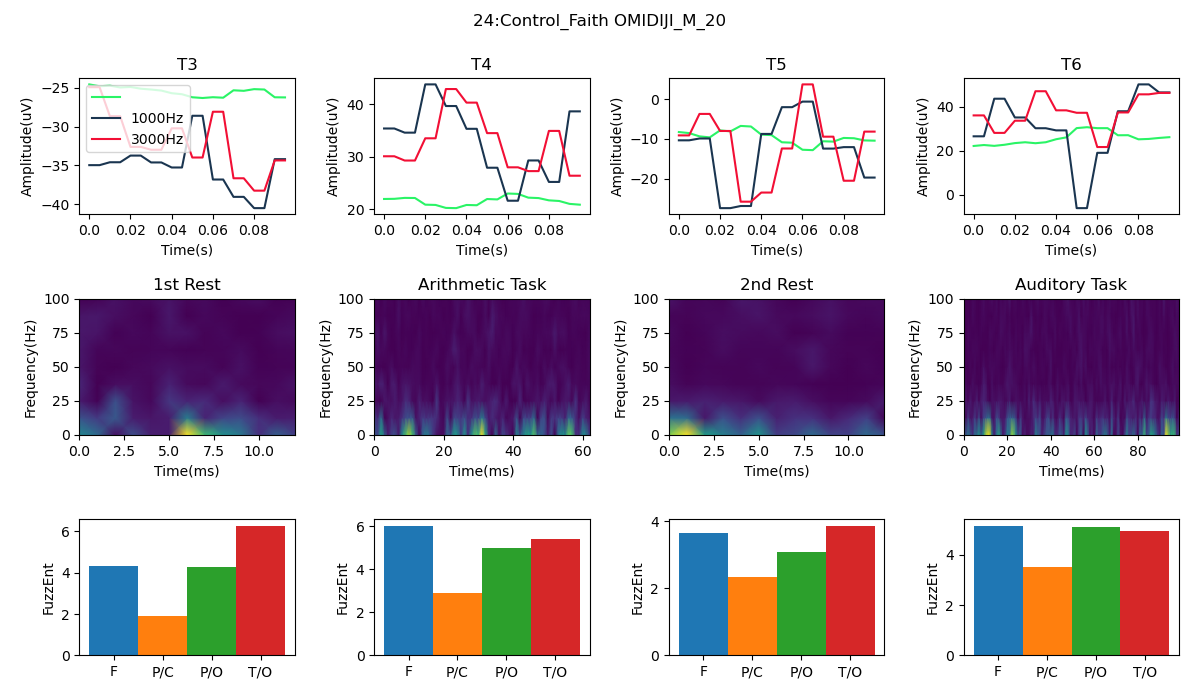
\includegraphics[width=\textwidth]{../../data_analysis_results/results/Control/24.png}
  \caption{Control 24}
  \label{fig:control_24}
\end{figure}
\clearpage
\begin{figure}
  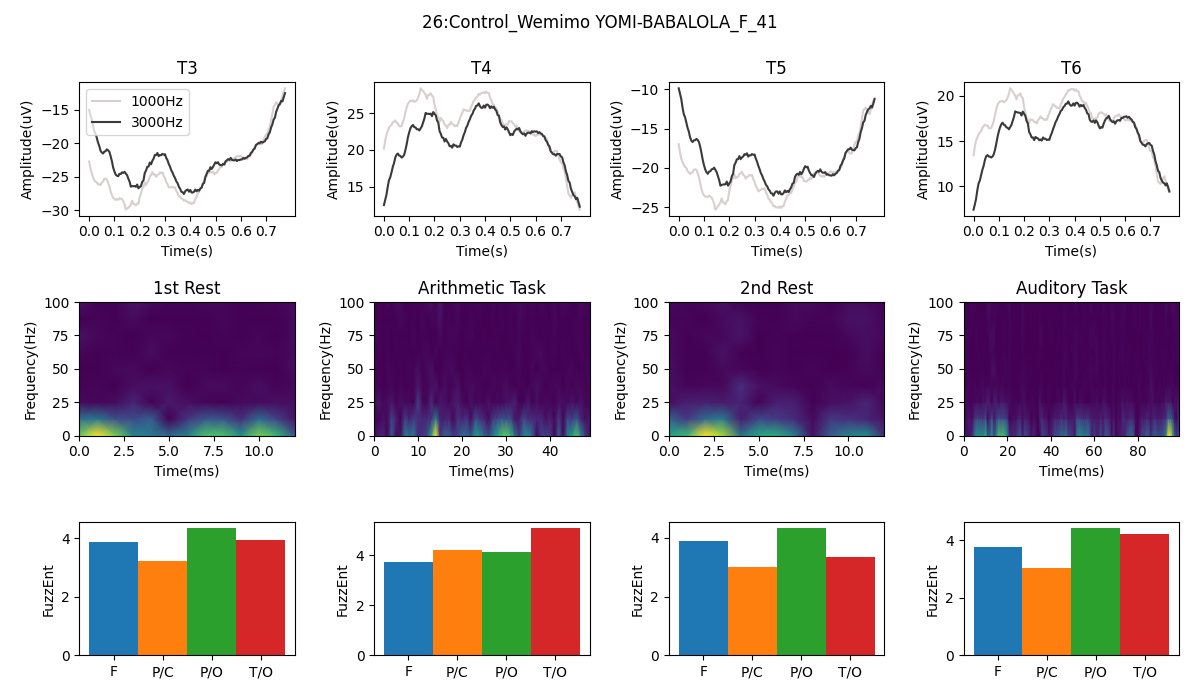
\includegraphics[width=\textwidth]{../../data_analysis_results/results/Control/26.png}
  \caption{Control 26}
  \label{fig:control_26}
\end{figure}
\clearpage
\begin{figure}
  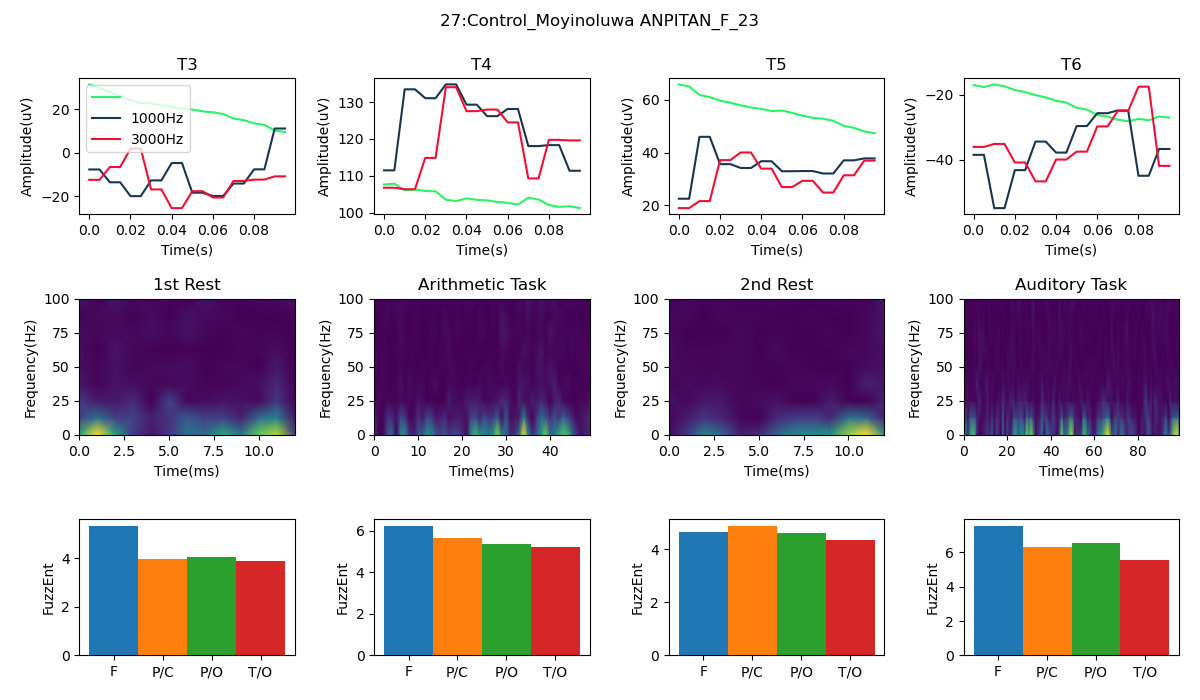
\includegraphics[width=\textwidth]{../../data_analysis_results/results/Control/27.png}
  \caption{Control 27}
  \label{fig:control_27}
\end{figure}
\clearpage
\begin{figure}
  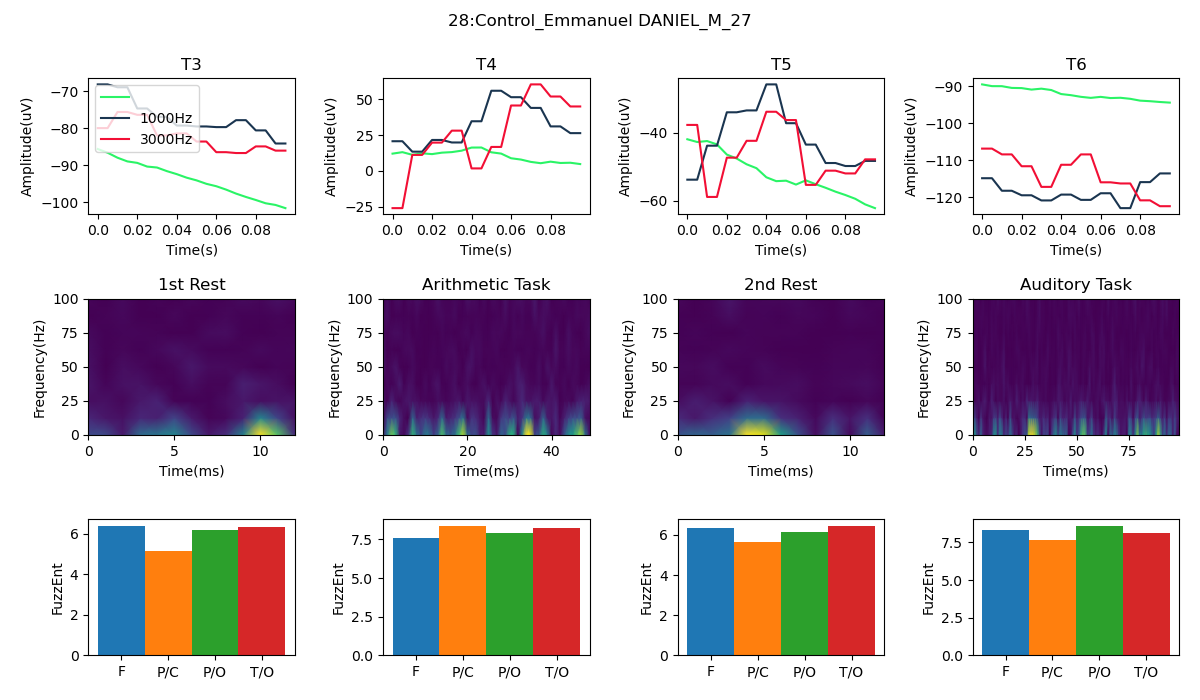
\includegraphics[width=\textwidth]{../../data_analysis_results/results/Control/28.png}
  \caption{Control 28}
  \label{fig:control_28}
\end{figure}
\clearpage
\begin{figure}
  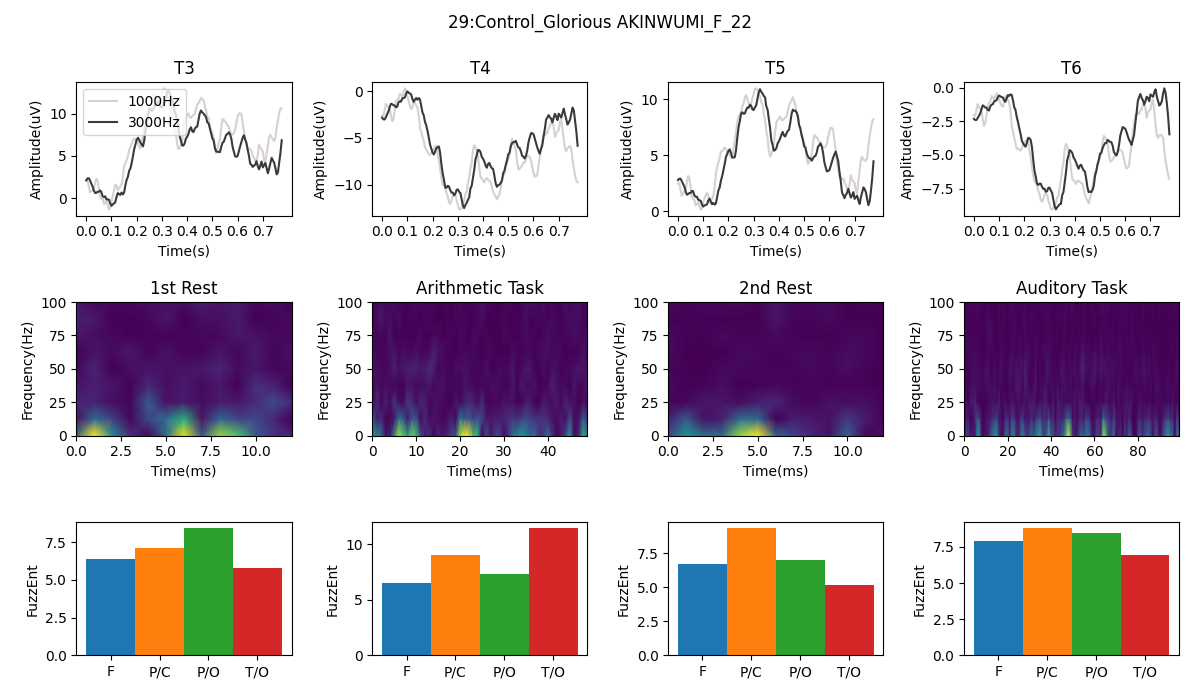
\includegraphics[width=\textwidth]{../../data_analysis_results/results/Control/29.png}
  \caption{Control 29}
  \label{fig:control_29}
\end{figure}
\clearpage
\begin{figure}
  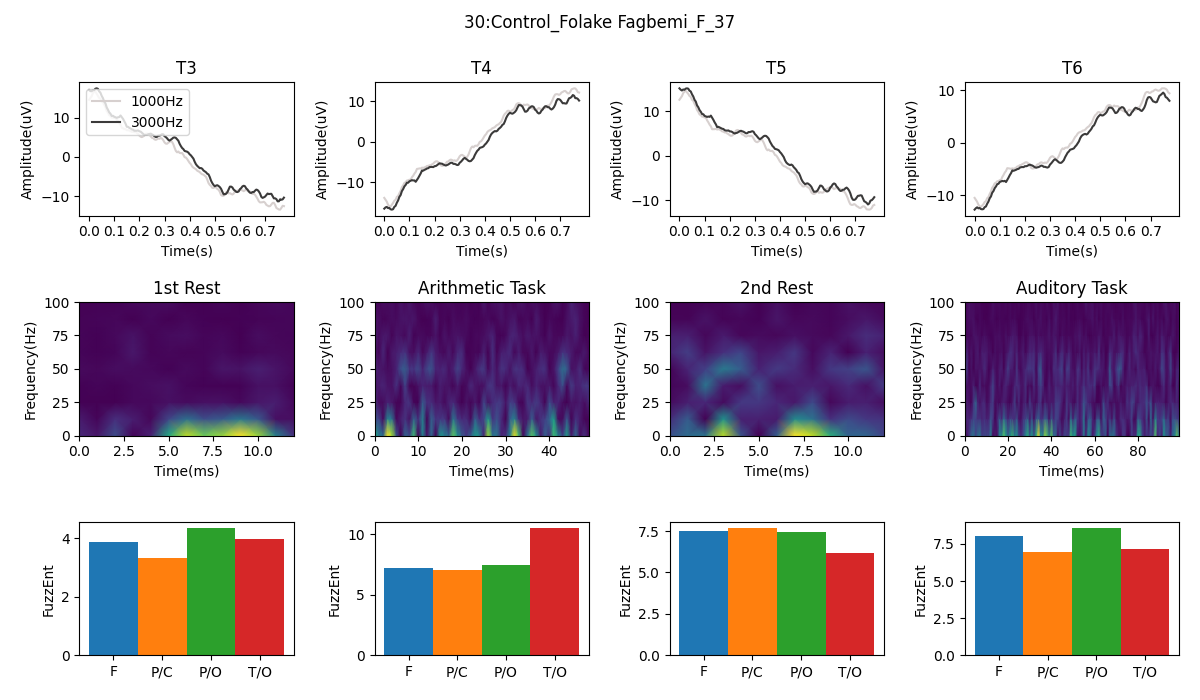
\includegraphics[width=\textwidth]{../../data_analysis_results/results/Control/30.png}
  \caption{Control 30}
  \label{fig:control_30}
\end{figure}
\clearpage
\begin{figure}
  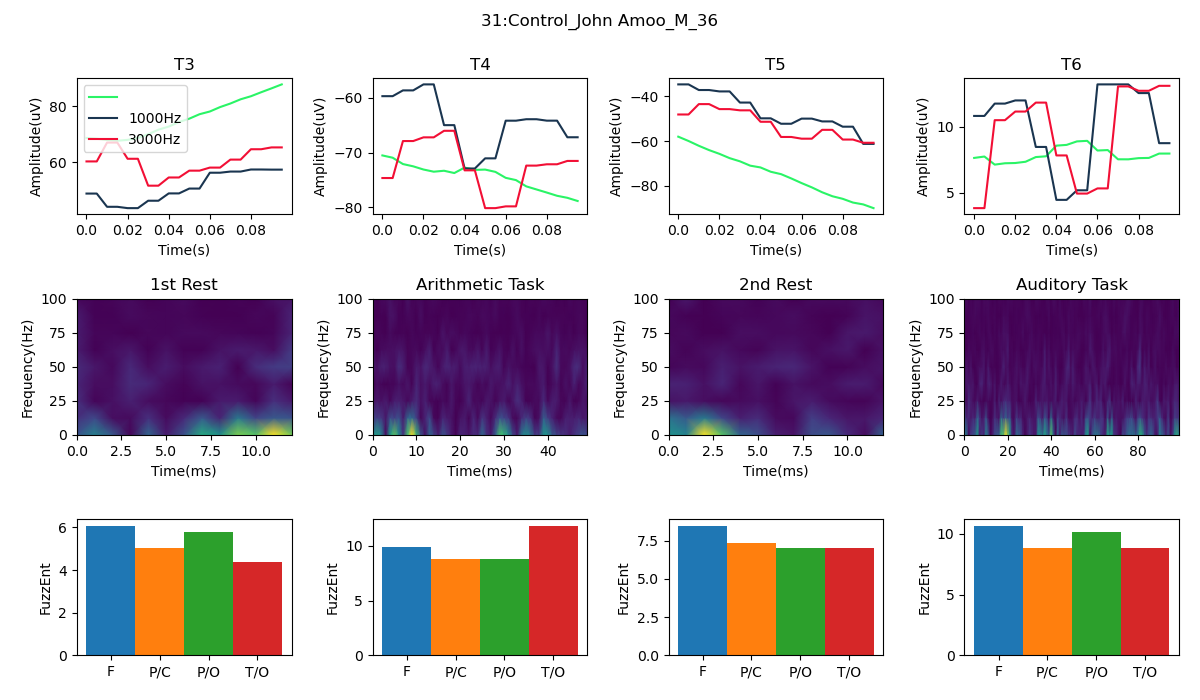
\includegraphics[width=\textwidth]{../../data_analysis_results/results/Control/31.png}
  \caption{Control 31}
  \label{fig:control_31}
\end{figure}

\clearpage
\begin{figure}
  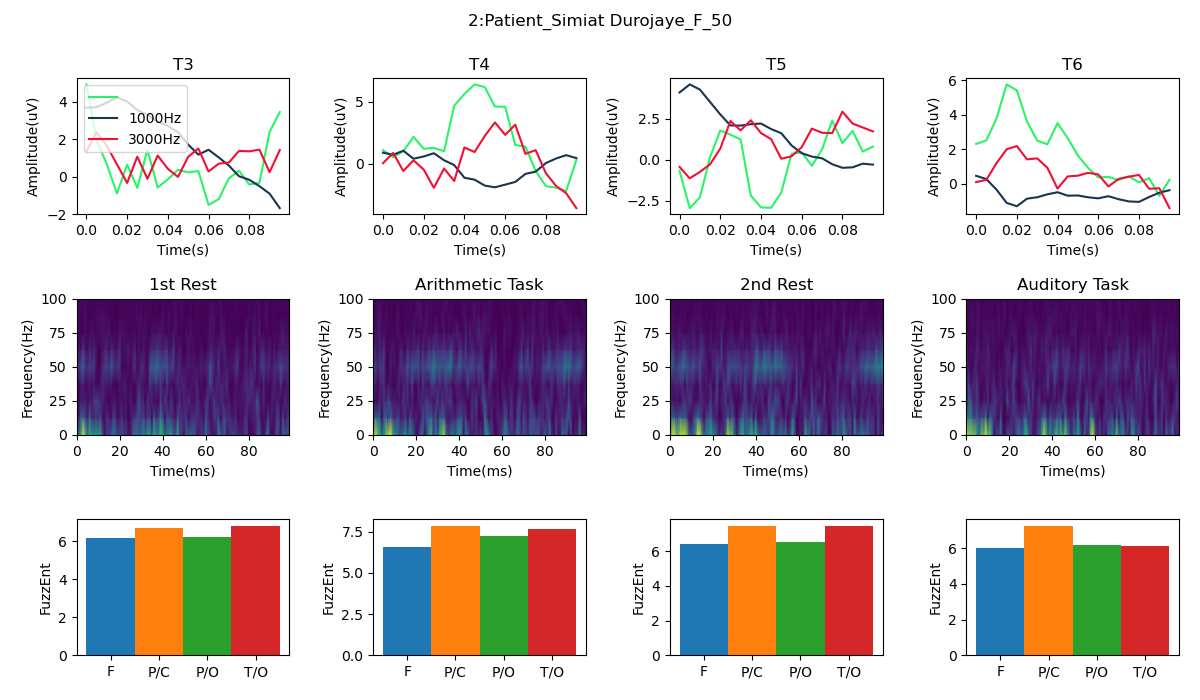
\includegraphics[width=\textwidth]{../../data_analysis_results/results/Patient/2.png}
  \caption{Patient 2}
  \label{fig:patient_2}
\end{figure}
\clearpage
\begin{figure}
  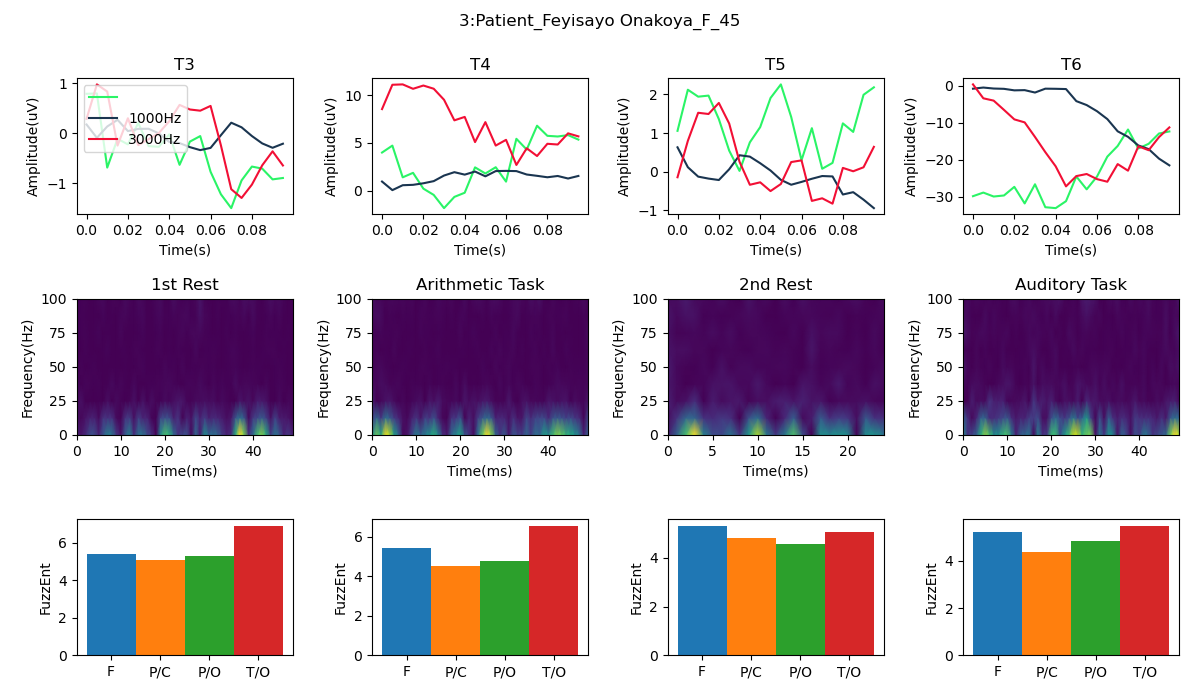
\includegraphics[width=\textwidth]{../../data_analysis_results/results/Patient/3.png}
  \caption{Patient 3}
  \label{fig:patient_3}
\end{figure}
\clearpage
\begin{figure}
  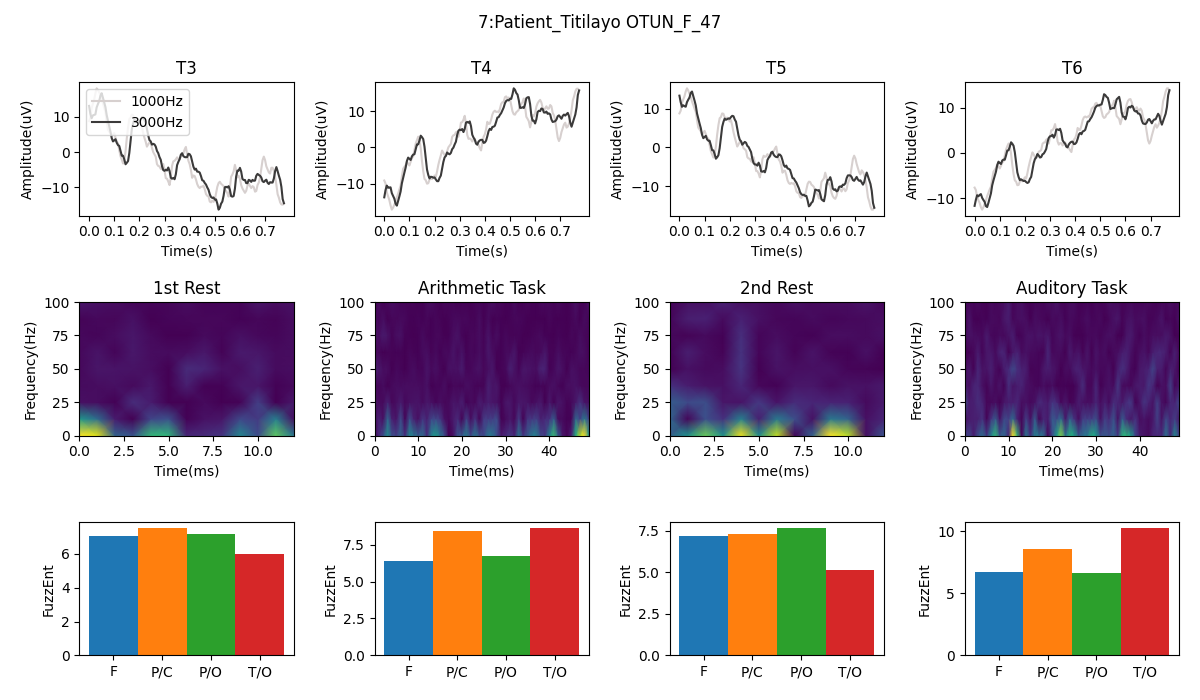
\includegraphics[width=\textwidth]{../../data_analysis_results/results/Patient/7.png}
  \caption{Patient 7}
  \label{fig:patient_7}
\end{figure}
\clearpage
\begin{figure}
  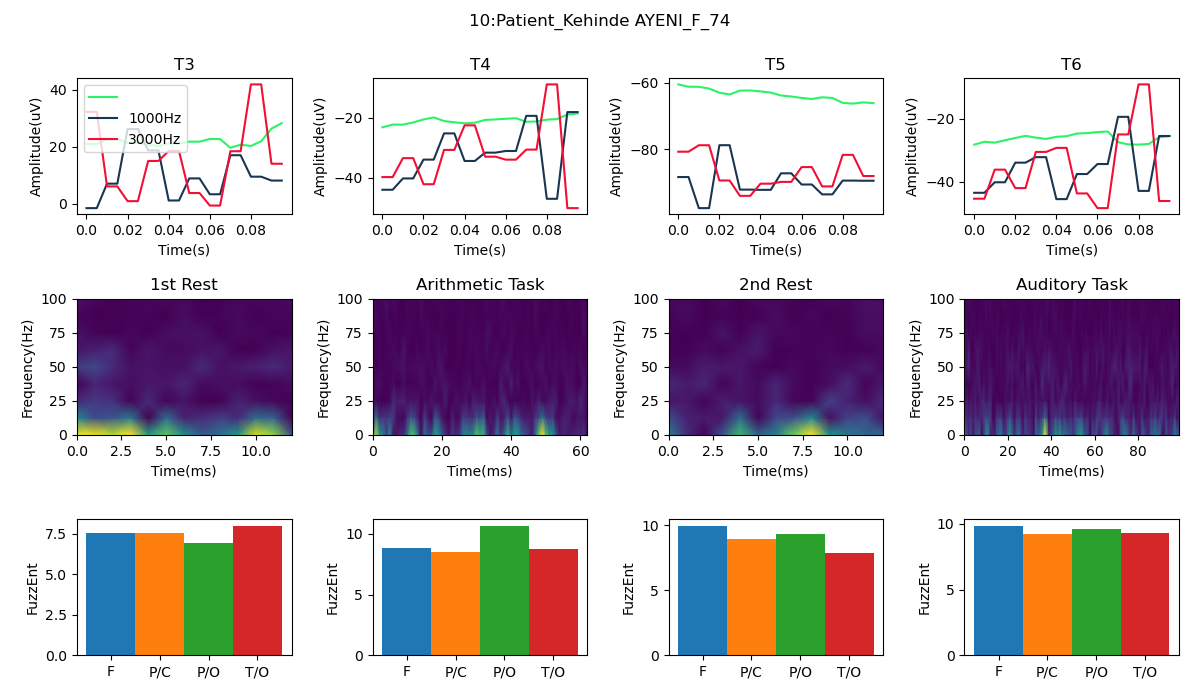
\includegraphics[width=\textwidth]{../../data_analysis_results/results/Patient/10.png}
  \caption{Patient 10}
  \label{fig:patient_10}
\end{figure}
\clearpage
\begin{figure}
  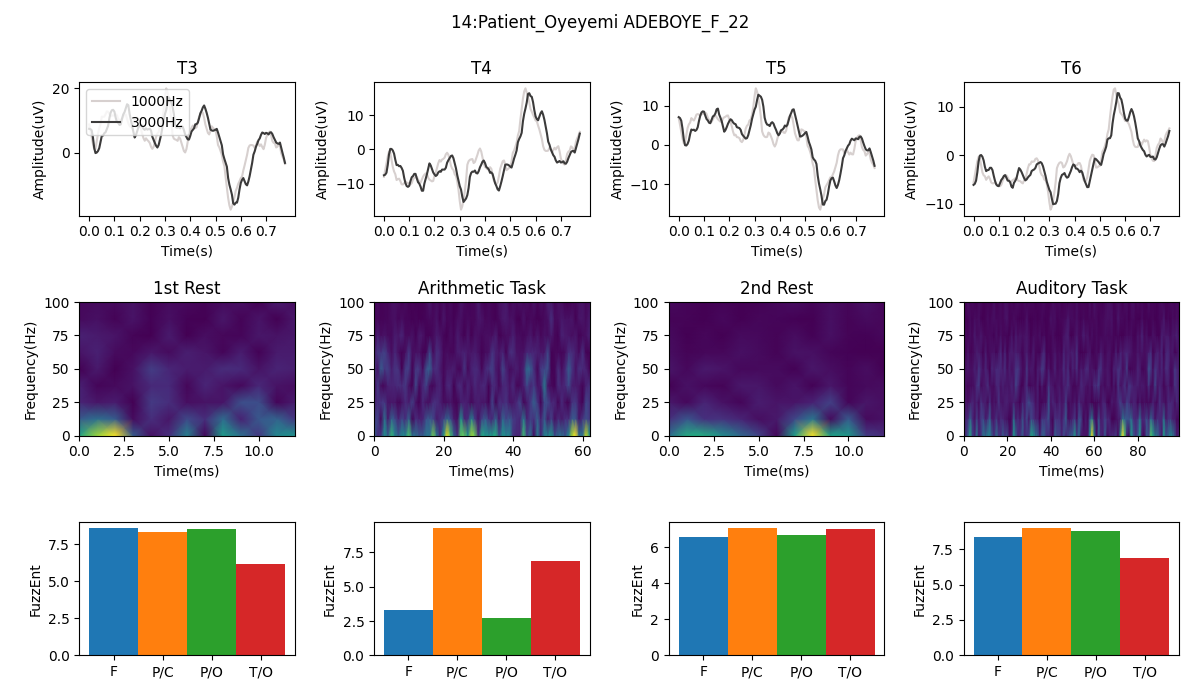
\includegraphics[width=\textwidth]{../../data_analysis_results/results/Patient/14.png}
  \caption{Patient 14}
  \label{fig:patient_14}
\end{figure}
\clearpage
\begin{figure}
  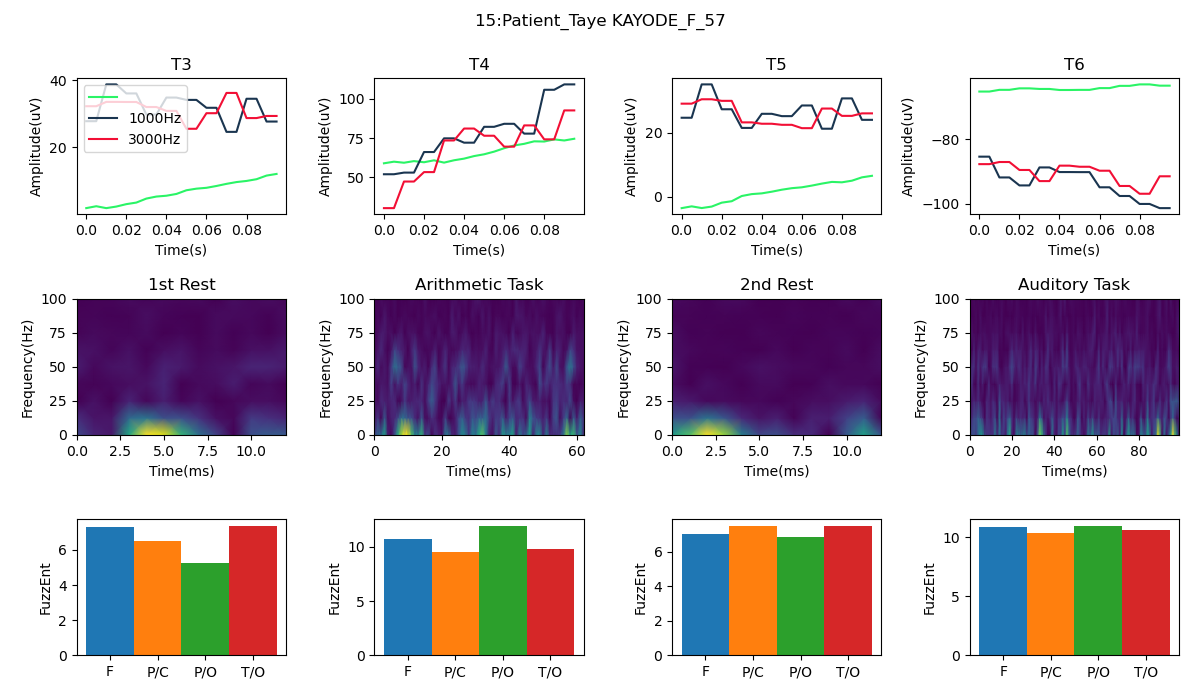
\includegraphics[width=\textwidth]{../../data_analysis_results/results/Patient/15.png}
  \caption{patient 15}
  \label{fig:patient_15}
\end{figure}
\clearpage
\begin{figure}
  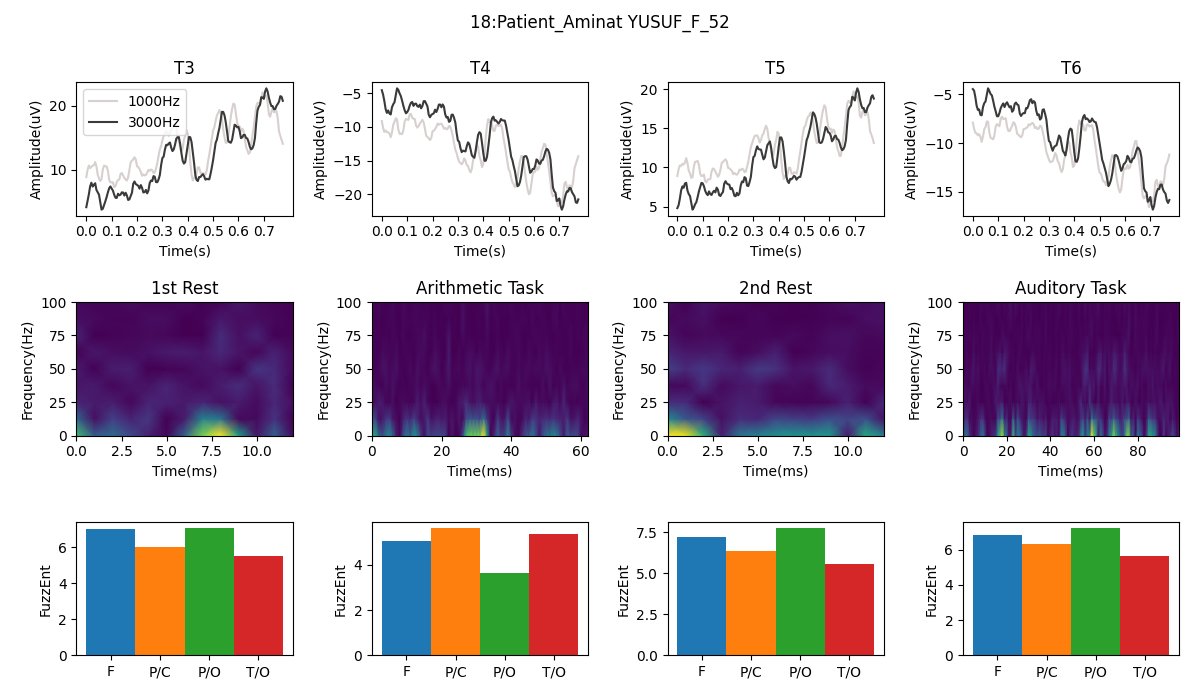
\includegraphics[width=\textwidth]{../../data_analysis_results/results/Patient/18.png}
  \caption{patient 18}
  \label{fig:patient_18}
\end{figure}
\clearpage
\begin{figure}
  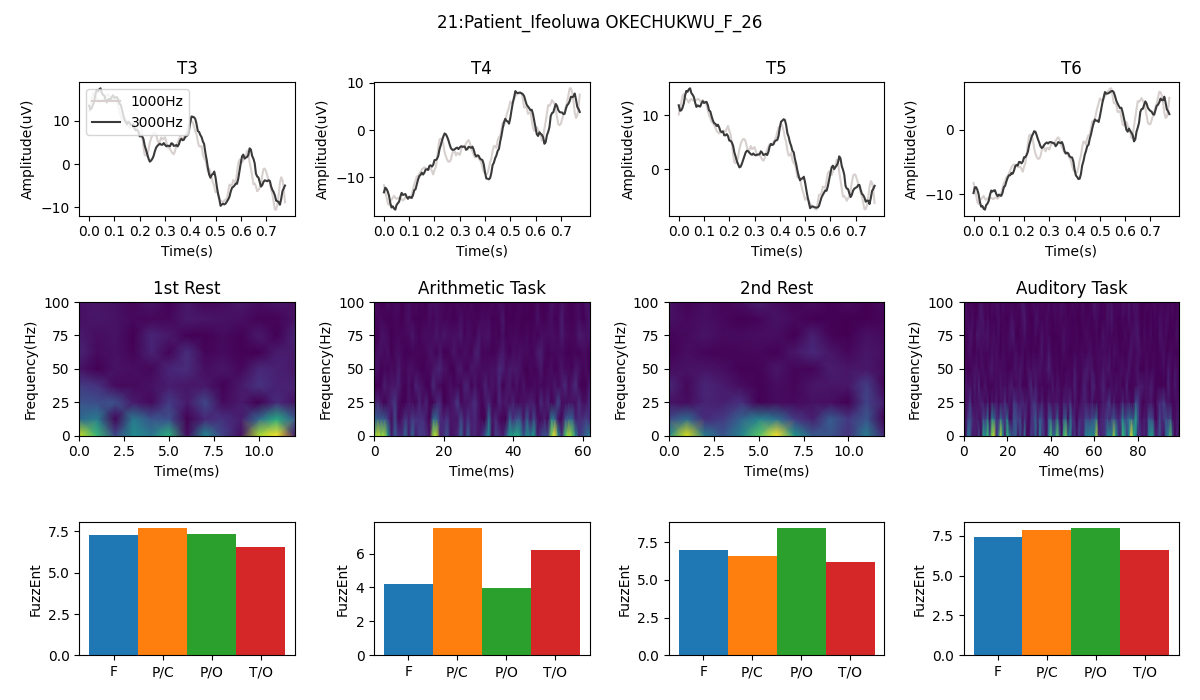
\includegraphics[width=\textwidth]{../../data_analysis_results/results/Patient/21.png}
  \caption{patient 21}
  \label{fig:patient_21}
\end{figure}
\clearpage
\begin{figure}
  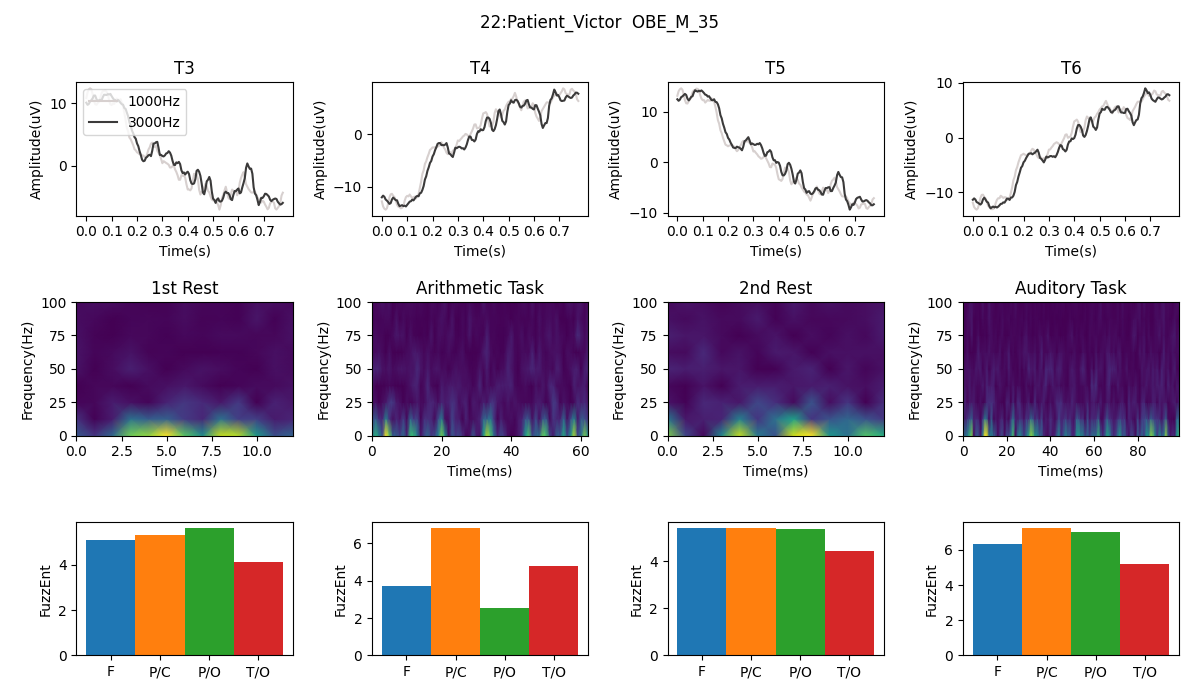
\includegraphics[width=\textwidth]{../../data_analysis_results/results/Patient/22.png}
  \caption{Patient 22}
  \label{fig:patient_22}
\end{figure}
\clearpage
\begin{figure}
  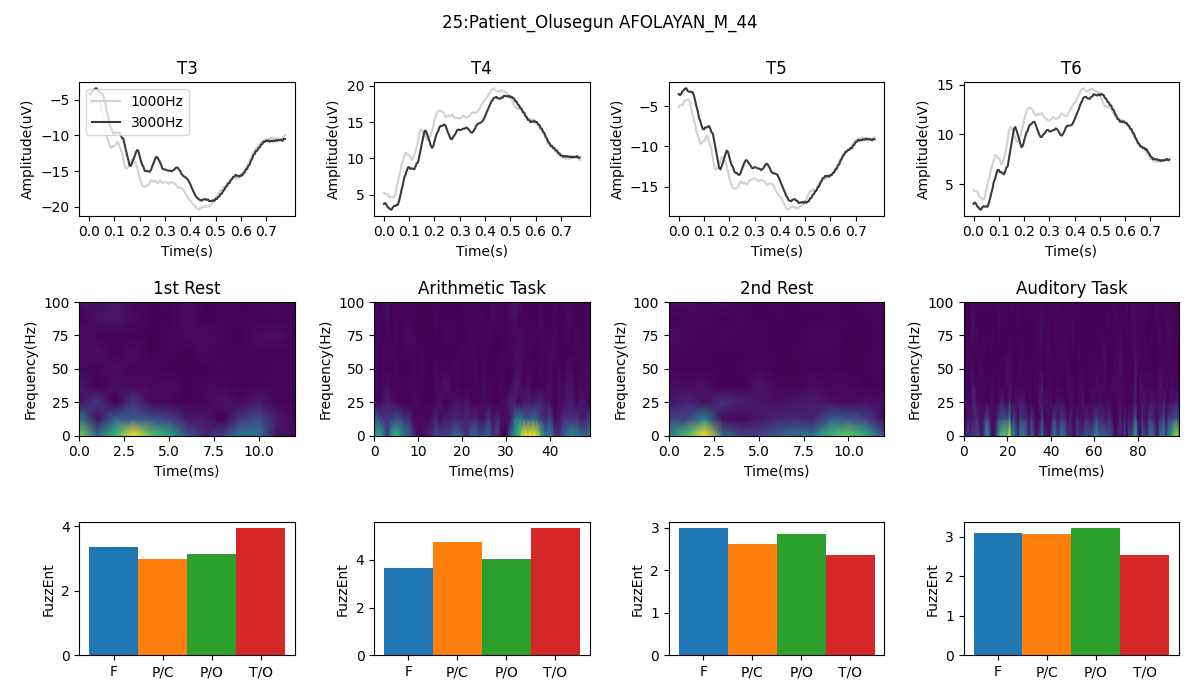
\includegraphics[width=\textwidth]{../../data_analysis_results/results/Patient/25.png}
  \caption{Patient 25}
  \label{fig:patient_25}
\end{figure}

\end{document}